\pagestyle{headings}
\chapter{Joint Distributions} \label{chp 5}
\thispagestyle{fancy}
\section{Joint Probability Mass Functions}

\begin{defn}\index{Joint Probability Mass Function}\index{Joint Distribution}\label{JointPMF}
If $X$ and $Y$ are discrete random variables, their joint probability mass function is given by $f_{X,Y}(x,y) = P(X = x  \cap Y = y)$.
\end{defn}
\par
The joint pmf takes an element from the sample space of $X$, another from the sample space of $Y$, and outputs the probability that both those outcomes occur.
\begin{examp}
Suppose a red die and a blue die are rolled. Let X denote the result on the red die, and Y the result on the blue die. The probability that both dice show six is $\frac{1}{36}$. Using the language of random variables, we can write this as $f_{X,Y}(6,6) = \frac{1}{36}$.
\end{examp}
\begin{examp}\label{DependentJointPMF}
Let $X$ be an integer between $1$ and $5$ inclusive, chosen uniformly at random, and let $Y$ be an integer between $X$ and $5$ inclusive, chosen uniformly at random. Compute $f_{X,Y}(3,5)$ and $f_{X,Y}(5,3)$.
$$f_{X,Y}(3,5) = P(X = 3 \cap  Y = 5) = P(X = 3)\cdot P(Y = 5 \given X = 3) = \textstyle\frac{1}{5}\cdot\frac{1}{3} = \frac{1}{15}$$
\noindent Note that $P(Y = 5 \given X = 3) = \frac{1}{3}$ since when $X = 3$, the distribution of $Y$ is uniform on $\{3,4,5\}$, so it takes each of those values with probability $\frac{1}{3}$.
$$f_{X,Y}(5,3) = P(X = 5 \cap  Y = 3) = P(X = 5)\cdot P(Y = 3 \given X = 5) = \textstyle\frac{1}{5}\cdot 0 = 0$$
Note that $P(Y = 3 \given X = 5) = 0$ above since when $X = 5$, $Y$ is uniform on the set containing only $\{5\}$, and hence $Y=3$ cannot occur.
\end{examp}
\par
We can visualize a joint pmf for two discrete random variables $X$ and $Y$ using a table or a bar graph over a two dimensional domain. The pmf $f_{X,Y}$ in Example \ref{DependentJointPMF} is shown below.
\begin{center}
\begin{minipage}{0.45\textwidth}
\renewcommand{\arraystretch}{1.5}
\begin{tabular}{c|ccccc}
$_{X} \setminus ^Y$ & $1$ & $2$ & $3$ & $4$ & $5$ \\
\hline
$1$ & $\frac{1}{25}$ & $\frac{1}{25}$ & $\frac{1}{25}$ & $\frac{1}{25}$ & $\frac{1}{25}$ \\
$2$ & $0$ & $\frac{1}{20}$ & $\frac{1}{20}$ & $\frac{1}{20}$ & $\frac{1}{20}$ \\
$3$ & $0$ & $0$ & $\frac{1}{15}$ & $\frac{1}{15}$ & $\frac{1}{15}$ \\
$4$ & $0$ & $0$ & $0$ & $\frac{1}{10}$ & $\frac{1}{10}$ \\
$5$ & $0$ & $0$ & $0$ & $0$ & $\frac{1}{5}$ \\
\end{tabular}
\renewcommand{\arraystretch}{1}
\end{minipage}\begin{minipage}{0.45\textwidth}
\newcommand{\myGlobalTransformation}[2]
{
    \pgftransformcm{1}{0}{0.4}{0.5}{\pgfpoint{#1cm}{#2cm}}
}
% draw a 4x4 helper grid in 3D
% Input: point of origins x and y coordinate and additional drawing-parameters
\newcommand{\gridThreeD}[3]
{
    \begin{scope}
        \myGlobalTransformation{#1}{#2};
        \draw [#3,step=1cm] grid (6,6);
    \end{scope}
}

\begin{tikzpicture}[scale = 0.7]

    %draws helper-grid:
    \gridThreeD{0}{0}{black!50};

    %draws lower graph lines and those in z-direction:
    \begin{scope}
        \myGlobalTransformation{0}{0};
        
        \draw[blue,thick, -{Circle[]}] (1,1) -- ++(-0.6,1.5) {};
        \draw[blue,thick, -{Circle[]}] (1,2) -- ++(-0.6,1.5) {};
        \draw[blue,thick, -{Circle[]}] (1,3) -- ++(-0.6,1.5) {};
        \draw[blue,thick, -{Circle[]}] (1,4) -- ++(-0.6,1.5) {};
        \draw[blue,thick, -{Circle[]}] (1,5) -- ++(-0.6,1.5) {};
        
        \draw[blue,thick, -{Circle[]}] (2,2) -- ++(-0.75,1.875) {};
        \draw[blue,thick, -{Circle[]}] (2,3) -- ++(-0.75,1.875) {};
        \draw[blue,thick, -{Circle[]}] (2,4) -- ++(-0.75,1.875) {};
        \draw[blue,thick, -{Circle[]}] (2,5) -- ++(-0.75,1.875) {};
        
        \draw[blue,thick, -{Circle[]}] (3,3) -- ++(-1,2.5) {};
        \draw[blue,thick, -{Circle[]}] (3,4) -- ++(-1,2.5) {};
        \draw[blue,thick, -{Circle[]}] (3,5) -- ++(-1,2.5) {};
        
        \draw[blue,thick, -{Circle[]}] (4,4) -- ++(-1.5,3.75) {};
        \draw[blue,thick, -{Circle[]}] (4,5) -- ++(-1.5,3.75) {};
        
        \draw[blue,thick, -{Circle[]}] (5,5) -- ++(-3,7.5) {};
        
        \node at (1.2,-0.7) {$1$};
        \node at (2.2,-0.7) {$2$};
        \node at (3.2,-0.7) {$3$};
        \node at (4.2,-0.7) {$4$};
        \node at (5.2,-0.7) {$5$};
        \node at (6.5,-0.7) {$X$};
        
        \node at (-0.5,1.2) {$1$};
        \node at (-0.5,2.2) {$2$};
        \node at (-0.5,3.2) {$3$};
        \node at (-0.5,4.2) {$4$};
        \node at (-0.5,5.2) {$5$};
        \node at (-0.5,6.5) {$Y$};
        
    \end{scope}

\end{tikzpicture}
\end{minipage}
\end{center}
\begin{example}\label{DieCoinJointPMF} Suppose we roll a die and whatever the result, flip a coin that number of times. Let $X$ be the result of die roll. Let $Y = 0$ if no heads were flipped, $Y=1$ if at least one head was flipped. Graph the joint pmf $f_{X,Y}$.
\par
\noindent Since $X$ takes values in the set $\{1,2,3,4,5,6\}$ and $Y$ takes values in $\{0,1\}$, we need to compute twelve probabilities, one for each pair of possible values. The computation of $f_{X,Y}(4,1)$ is shown below, and the rest are left as an exercise.
$$\begin{aligned}f_{X,Y}(4,1) &= P(X = 4 \cap  Y = 1) \\ 
&= P(X=4)\cdot P(Y = 1 \given X = 4) \\
& = \textstyle\frac{1}{6} \cdot \left(1 - \left(\textstyle\frac{1}{2}\right)^{4}\right) = \frac{15}{96}\end{aligned}$$
\noindent Note that $P(Y = 1 \given X = 4)$ is the probability of observing at least one head in four independent flips of a coin, which was calculated using the complement rule.

\begin{center}
\hspace*{0.5in}\begin{minipage}{0.2\textwidth}
\centering
\renewcommand{\arraystretch}{1.5}
\begin{tabular}{c|cc}
$_{X} \setminus ^Y$ & $0$ & $1$ \\
\hline
$1$ & $\frac{1}{12}$ & $\frac{1}{12}$ \\
$2$ & $\frac{1}{24}$ & $\frac{3}{24}$ \\
$3$ & $\frac{1}{48}$ & $\frac{7}{48}$ \\
$4$ & $\frac{1}{96}$ & $\frac{15}{96}$ \\
$5$ & $\frac{1}{192}$ & $\frac{31}{192}$ \\
$6$ & $\frac{1}{384}$ & $\frac{63}{384}$ \\
\end{tabular}
\renewcommand{\arraystretch}{1}
\end{minipage}\begin{minipage}{0.7\textwidth}
\centering
\newcommand{\myGlobalTransformation}[2]
{
    \pgftransformcm{1}{0}{0.4}{0.5}{\pgfpoint{#1cm}{#2cm}}
}
% draw a 4x4 helper grid in 3D
% Input: point of origins x and y coordinate and additional drawing-parameters
\newcommand{\gridThreeD}[3]
{
    \begin{scope}
        \myGlobalTransformation{#1}{#2};
        \draw [#3,step=1cm] grid (7,3);
    \end{scope}
}

\begin{tikzpicture}[scale = 0.7]

    %draws helper-grid:
    \gridThreeD{0}{0}{black!50};

    %draws lower graph lines and those in z-direction:
    \begin{scope}
        \myGlobalTransformation{0}{0};
        
        \draw[blue,thick, -{Circle[]}] (1,1) -- ++(-1.33,3.33) {};
        \draw[blue,thick, -{Circle[]}] (1,2) -- ++(-1.33,3.33) {};
        
        \draw[blue,thick, -{Circle[]}] (2,1) -- ++(-0.66,1.66) {};
        \draw[blue,thick, -{Circle[]}] (2,2) -- ++(-2,5) {};
        
        \draw[blue,thick, -{Circle[]}] (3,1) -- ++(-0.33,0.83) {};
        \draw[blue,thick, -{Circle[]}] (3,2) -- ++(-2.33,5.83) {};
        
        \draw[blue,thick, -{Circle[]}] (4,1) -- ++(-0.16,0.42) {};
        \draw[blue,thick, -{Circle[]}] (4,2) -- ++(-2.5,6.25) {};
        
        \draw[blue,thick, -{Circle[]}] (5,1) -- ++(-0.10,0.24) {};
        \draw[blue,thick, -{Circle[]}] (5,2) -- ++(-2.60,6.44) {};
        
        \draw[blue,thick, -{Circle[]}] (6,1) -- ++(-0.08,0.20) {};
        \draw[blue,thick, -{Circle[]}] (6,2) -- ++(-2.62,6.56) {};
        
        \node at (1.2,-0.7) {$1$};
        \node at (2.2,-0.7) {$2$};
        \node at (3.2,-0.7) {$3$};
        \node at (4.2,-0.7) {$4$};
        \node at (5.2,-0.7) {$5$};
        \node at (6.2,-0.7) {$6$};
        \node at (7.5,-0.7) {$X$};
        
        \node at (-0.5,1.2) {$0$};
        \node at (-0.5,2.2) {$1$};
        \node at (-0.5,3.5) {$Y$};
        
    \end{scope}

\end{tikzpicture}
\end{minipage}
\end{center}
\end{example}
\par
Any finite sequence of discrete random variables $X_1, X_2, \, \dots \, , X_n$ determines a joint pmf $f_{X_1, X_2, \, \dots \, , X_n}$, and $f_{X_1, X_2, \, \dots \, , X_n}(x_1,x_2,\,\dots\, ,x_n)$ denotes the probability of the event $X_1 = x_1 \cap X_2 = x_2 \cap \, \dots \, \cap X_n = x_n$.
\par
Our method of visualizing a joint pmf no longer applies for sequences of more than two random variables, as we run out of spatial dimensions. Nonetheless, the probability calculations involved should look familiar.
\begin{example}
Two cards are drawn without replacement from a shuffled standard deck. Among the two chosen cards, let $X$ denote the number of black cards, $Y$ denote the number of hearts, and $Z$ denote the number of spades. Find $f_{X,Y,Z}(2,0,1)$.
\par
\noindent We want the probability of drawing two black cards, exactly one of which is a spade. This can occur in two ways, by drawing a spade followed by a club, or a club followed by a spade. These two options are mutually exclusive, so we sum their probabilities.
$$f_{X,Y,Z}(2,0,1) = \frac{13}{52} \cdot \frac{13}{51} + \frac{13}{52} \cdot \frac{13}{51} = \frac{338}{2652}$$
\end{example}

\subsection*{Continuous Joint Distributions}

The idea of a joint distribution for two discrete random variables can be extended to the case where both those random variables are continuous in a natural way. 
\par
The joint probability density function for a pair of continuous random variables $X$ and $Y$ is a non-negative function $f_{X,Y}(x,y)$ such that for any pair of intervals $[a,b]$ and $[c,d]$, the probability $X \in [a,b]$ and $Y \in [c,d]$ is given by the volume of the region underneath the graph of $f_{X,Y}$ on the rectangle $[a,b] \times [c,d]$.

\begin{center}
\newcommand{\myGlobalTransformation}[2]
{
    \pgftransformcm{1}{0}{0.4}{0.5}{\pgfpoint{#1cm}{#2cm}}
}
% draw a 4x4 helper grid in 3D
% Input: point of origins x and y coordinate and additional drawing-parameters
\newcommand{\gridThreeD}[3]
{
    \begin{scope}
        \myGlobalTransformation{#1}{#2};
        \draw [#3,step=1cm] grid (6,3);
    \end{scope}
}

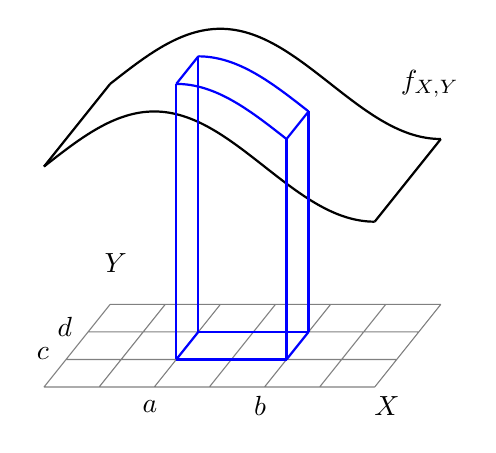
\begin{tikzpicture}[scale = 0.7]

    %draws helper-grid:
    \gridThreeD{0}{0}{black!50};

    %draws pdf
    \draw[x=0.5cm,y=1cm, thick, black] 
        (0,4) sin (4,5) cos (8,4) sin (12,3);
    \draw[x=0.5cm,y=1cm, thick, black] 
        (2.4,5.5) sin (6.4,6.5) cos (10.4,5.5) sin (14.4,4.5);
    \draw[x=0.5cm,y=1cm, thick, black] 
        (0,4) -- (2.4,5.5);
    \draw[x=0.5cm,y=1cm, thick, black] 
        (12,3) -- (14.4,4.5);
        
    %draws trapezoidy top
    \draw[x=0.5cm,y=1cm, thick, blue] 
        (4.8,5.5) -- (5.6,6);
    \draw[x=0.5cm,y=1cm, thick, blue] 
        (8.8,4.5) -- (9.6,5);
   \draw[x=0.5cm,y=1cm, thick, blue] 
        (4.8,5.5) cos (8.8,4.5);
    \draw[x=0.5cm,y=1cm, thick, blue] 
        (5.6,6) cos (9.6,5);
        
    %draws trapezoidy sides
    \draw[x=0.5cm,y=1cm, thick, blue] 
        (4.8,0.5) -- (4.8,5.5);
    \draw[x=0.5cm,y=1cm, thick, blue] 
        (8.8,0.5) -- (8.8,4.5);
    \draw[x=0.5cm,y=1cm, thick, blue] 
        (9.6,1) -- (9.6,5);
    \draw[x=0.5cm,y=1cm, thick, blue] 
        (5.6,1) -- (5.6,6);
        
     %draws trapezoidy bottom
     \draw[x=0.5cm,y=1cm, thick, blue] 
        (4.8,0.5) -- (8.8,0.5);
     \draw[x=0.5cm,y=1cm, thick, blue] 
        (8.8,0.5) -- (9.6,1);
     \draw[x=0.5cm,y=1cm, thick, blue] 
        (9.6,1) -- (5.6,1);
     \draw[x=0.5cm,y=1cm, thick, blue] 
        (5.6,1) -- (4.8,0.5);
        
    \node at (7,5.5) {$f_{X,Y}$};

    %draws lower graph lines and those in z-direction:
    \begin{scope}
        \myGlobalTransformation{0}{0};
        
        \node at (2.2,-0.7) {$a$};
        \node at (4.2,-0.7) {$b$};
        \node at (6.5,-0.7) {$X$};
       
        \node at (-0.5,1.2) {$c$};
        \node at (-0.5,2.2) {$d$};
        \node at (-0.5,4.5) {$Y$};
        
    \end{scope}

\end{tikzpicture}
\end{center}

If the graph of $f_{X,Y}$ above $[a,b] \times [c,d]$ is a plane, we could evaluate the volume of this blue region using elementary geometric methods, but in general this task will require some knowledge of multivariable calculus, which is beyond the scope of this course. 
\par
For this reason, we'll only discuss discrete joint distributions here. Rest assured that all the key definitions and results in this chapter have appropriate continuous analogues. If you're taking multivariable calculus, you can read about continuous joint distributions in \cite{StewartMultivariable} and \cite{Ghahramani}.

\section{Marginal Distributions}

If we're given the joint pmf $f_{X,Y}$ for two discrete random variables $X$ and $Y$, we can recover the distribution of $X$ alone in a straightforward way, by summing up probabilities in the table of $f_{X,Y}$.

\begin{examp} As in Example \ref{DependentJointPMF}, let $X$ be uniformly distributed on $\{1,2,3,4,5\}$ and let $Y$ be uniformly distributed on the set of whole numbers between X and 5 inclusive. We can recover the distribution of $X$ from the joint pmf $f_{X,Y}$ by summing along rows, since each row represents one possible value of $X$.

\begin{center}
\renewcommand{\arraystretch}{1.5}
\begin{tabular}{c|cccccc}
$_{X} \setminus ^Y$ & $1$ & $2$ & $3$ & $4$ & $5$  & \\
\cline{1-6}
$1$ & $\frac{1}{25}$ & $\frac{1}{25}$ & $\frac{1}{25}$ & $\frac{1}{25}$ & $\frac{1}{25}$ & ${\rightarrow}\ \ \frac{1}{5}$ \\
$2$ & $0$ & $\frac{1}{20}$ & $\frac{1}{20}$ & $\frac{1}{20}$ & $\frac{1}{20}$ & ${\rightarrow}\ \ \frac{1}{5}$ \\
$3$ & $0$ & $0$ & $\frac{1}{15}$ & $\frac{1}{15}$ & $\frac{1}{15}$ & ${\rightarrow}\ \ \frac{1}{5}$ \\
$4$ & $0$ & $0$ & $0$ & $\frac{1}{10}$ & $\frac{1}{10}$ & ${\rightarrow}\ \ \frac{1}{5}$ \\
$5$ & $0$ & $0$ & $0$ & $0$ & $\frac{1}{5}$  & ${\rightarrow}\  \ \frac{1}{5}$\\
\end{tabular}
\renewcommand{\arraystretch}{1}
\end{center}

\noindent As expected, the distribution we recover is uniform on the set $\{1,2,3,4,5\}$. 
\par
\noindent Similarly, since each column represents a possible value for $Y$, we can recover the distribution of $Y$ by summing along the columns. Note that higher values for $Y$ are more likely, which makes sense in this context.

\begin{center}
\renewcommand{\arraystretch}{1.5}
\begin{tabular}{c|ccccc}
$_{X} \setminus ^Y$ & $1$ & $2$ & $3$ & $4$ & $5$ \\
\cline{1-6}
$1$ & $\frac{1}{25}$ & $\frac{1}{25}$ & $\frac{1}{25}$ & $\frac{1}{25}$ & $\frac{1}{25}$  \\
$2$ & $0$ & $\frac{1}{20}$ & $\frac{1}{20}$ & $\frac{1}{20}$ & $\frac{1}{20}$ \\
$3$ & $0$ & $0$ & $\frac{1}{15}$ & $\frac{1}{15}$ & $\frac{1}{15}$  \\
$4$ & $0$ & $0$ & $0$ & $\frac{1}{10}$ & $\frac{1}{10}$ \\
$5$ & $0$ & $0$ & $0$ & $0$ & $\frac{1}{5}$ \\
\end{tabular}\\
\begin{tabular}{cccccc}
& $\downarrow$ & \hspace*{-0.1cm}$\downarrow$ & \hspace*{-0.05cm}$\downarrow$ & \hspace*{-0.2cm} $\downarrow$ & \hspace*{-0.2cm}$\downarrow$ \\
\hspace{0.8cm} & $\frac{1}{25}$ & \hspace*{-0.2cm} $\frac{9}{100}$ \hspace*{-0.1cm}& \hspace*{-0.15cm}$\frac{47}{300}$\hspace*{-0.1cm} &  \hspace*{-0.15cm} $\frac{77}{300}$  \hspace*{-0.1cm} & \hspace*{-0.2cm}$\frac{137}{300}$ \hspace*{-0.1cm} \\
\end{tabular}
\renewcommand{\arraystretch}{1}
\end{center}
\end{examp}

\begin{defn}\index{Marginal Distribution}\index{Distribution!Marginal}
Given the joint pmf $f_{X,Y}$ for discrete random variables $X$ and $Y$, the distribution of $X$ itself and the distribution of $Y$ itself are called marginal distributions. These distributions can be recovered by summing over all values of the other variable.
$$f_X(x) = \sum_{y} f_{X,Y}(x,y) \qquad f_Y(y) = \sum_{x} f_{X,Y}(x,y)$$
\end{defn}

\begin{examp}Consider the joint pmf $f_{X,Y}$ given in Example \ref{DieCoinJointPMF}. Calculate $f_{Y}(0)$ and $f_Y(1)$, then graph the marginal distribution of $Y$.
$$f_Y(0) = \sum_{x} f_{X,Y}(x,0) = \frac{1}{12} + \frac{1}{24} + \frac{1}{48} + \frac{1}{96} + \frac{1}{192} + \frac{1}{384} = \frac{63}{384}$$
$$f_Y(1) = \sum_{x} f_{X,Y}(x,1) = \frac{1}{12} + \frac{3}{24} + \frac{7}{48} + \frac{15}{96} + \frac{31}{192} + \frac{63}{384} = \frac{321}{384} $$
The graph of the pmf $f_Y$ is given below.
\begin{center}
\begin{tikzpicture}[scale = 0.7]
\begin{axis} [ymin = 0, ymax = 1, xmin = -1, xmax = 2,
		y tick label style={
        /pgf/number format/.cd,
            fixed,
            precision=2,
        /tikz/.cd
    }, ytick = {0.2,0.4,0.6,0.8,1}, xtick = {0,1}]
\addplot+[ycomb] plot coordinates {(0, 0.164) (1, 0.836)}; 
\end{axis}
\end{tikzpicture}
\end{center}
\end{examp}

\section{Independent Random Variables}

In Section \ref{IndependenceOfEvents}, we introduced the definition of independence for two events $A$ and $B$ over a sample space $\Omega$, and showed that two such events are independent when the probability that $A$ and $B$ both occur is the product of their probabilities.
\par
This notion of independence can be extended to discrete random variables by calling two random variables independent when for any possible values $x$ of $X$ and $y$ of $Y$, $f_{X,Y}(x,y) = P(X = x \cap  Y = y) = P(X = x)P(Y = y) = f_{X}(x)f_Y(y)$.

\begin{defn}\index{Independent Random Variables}\index{Independence!of random variables}\label{independentrvdef}
Two random variables $X$ and $Y$ are independent when their joint density function $f_{X,Y}$ is the product of the marginal distributions $f_X$ and $f_Y$. That is, for all possible values $x$ of $X$ and $y$ of $Y$, 
$$f_{X,Y}(x,y) = f_{X}(x)f_Y(y).$$
\end{defn}

\begin{thm}\label{independenceinfo}If $X$ and $Y$ are independent, knowledge of the value of $X$ provides no information about the value of $Y$, and vice-versa. That is, $P(Y = y \given X = x) = P(Y = y)$ and $P(X = x \given Y = y) = P(X = x)$ whenever both sides are defined.
\end{thm}
\begin{pf} Using the definition of conditional probability (Definition \ref{conditionalprob}), we have
$$\begin{aligned}P(Y = y \given X = x) &= \frac{P(Y = y \cap  X = x)}{P(X = x)} = \frac{P(X = x \cap  Y = y)}{P(X = x)} \\ &= \frac{f_{X,Y}(x,y)}{f_X(x)} = \frac{f_X(x)f_Y(y)}{f_X(x)} = f_Y(y) = P(Y = y). \end{aligned}$$
If the roles of $X$ and $Y$ are swapped, the same argument shows $P(X = x \given Y = y) = P(X = x)$. Note that division by zero is not a problem above, since if $P(X = x) = 0$ the conditional probability $P(Y = y \given X = x)$ is undefined.
\end{pf}

\begin{examp}Suppose that two cards are drawn with replacement from a shuffled deck. Let $X$ denote the number of hearts and $Y$ the number of black cards. Find the joint pmf $f_{X,Y}$ and the two marginal distributions. Are $X$ and $Y$ independent?
\par
\noindent The joint pmf is given in the table on the left, with the marginal distributions of $X$ and $Y$ on the right. 

\begin{center}
\begin{minipage}{0.4\textwidth}
\renewcommand{\arraystretch}{1.5}
\centering
\begin{tabular}{c|ccccc}
$_{X} \setminus ^Y$ & $0$ & $1$ & $2$ \\
\hline
$0$ & $\frac{1}{16}$ & $\frac{4}{16}$ & $\frac{4}{16}$ \\
$1$ & $\frac{2}{16}$ & $\frac{4}{16}$ & $0$ \\
$2$ & $\frac{1}{16}$ & $0$ & $0$  \\
\end{tabular}
\end{minipage}\begin{minipage}{0.25\textwidth}
\centering
\renewcommand{\arraystretch}{1.5}
\begin{tabular}{c|c}
$x$ & $f_X(x)$ \\
\hline
$0$ & $\frac{9}{16}$ \\
$1$ & $\frac{6}{16}$ \\
$2$ & $\frac{1}{16}$ \\
\end{tabular}
\end{minipage}\begin{minipage}{0.25\textwidth}
\centering
\renewcommand{\arraystretch}{1.5}
\begin{tabular}{c|c}
$y$ & $f_Y(y)$ \\
\hline
$0$ & $\frac{1}{4}$ \\
$1$ & $\frac{1}{2}$ \\
$2$ & $\frac{1}{4}$ \\
\end{tabular}
\end{minipage}
\end{center}
The random variables $X$ and $Y$ are not independent, since, for instance, $f_{X,Y}(2,1)$ is zero while $f_X(2)f_Y(1) = \frac{1}{16}\cdot\frac{1}{2} = \frac{1}{32}$.
\end{examp}
\par
Note that in the last example, we would expect $X$ and $Y$ are not independent, since information about whether the two cards drawn were hearts should certainly influence our beliefs about whether they were black.
\par
This kind of reasoning about independence is formalized in Theorem \ref{independenceinfo}, but be warned that incorrectly concluding independence based on informal reasoning is a very common error. The definition of independence makes no reference to any real-world connection or lack thereof between the quantities in question.
\par
The definition of independence above extends immediately to sequences of more than two random variables. The sequence $X_1, X_2,\,\dots\,, X_n$ is said to be independent\index{Independence!of a sequence of random variables} when $f_{X_1, X_2, \,\dots\, , X_n}(x_1, x_2, \,\dots\, , x_n) = f_{X_1}(x_1)f_{X_2}(x_2) \,\dots\, f_{X_n}(x_n)$, that is, when the joint pmf is the product of the marginal distributions.

\subsection*{Sums of Independent Random Variables}

To conclude our study of joint distributions, we'll investigate the distribution of $X+Y$ when $X$ and $Y$ are independent random variables. Our knowledge of this `sum distribution' will become very valuable when we start statistics.
\par

\begin{examp}\label{sumdistribution}Suppose $X$ and $Y$ are independent with $X \sim Binomial(3,\frac{1}{5})$ and $Y \sim Binomial(2,\frac{1}{2})$. If $S = X + Y$, determine the distribution of S.
\par
\noindent Since we're given that $X$ and $Y$ are independent, we have $f_{X,Y}(x,y)  = f_X(x)f_Y(y)$, so we can reconstruct the joint pmf $f_{X,Y}$ by multiplication.

\begin{center}
\begin{minipage}{0.25\textwidth}
\centering
\renewcommand{\arraystretch}{1.5}
\begin{tabular}{c|c}
$x$ & $f_X(x)$ \\
\hline
$0$ & $\frac{64}{125}$ \\
$1$ & $\frac{48}{125}$ \\
$2$ & $\frac{12}{125}$ \\
$3$ & $\frac{1}{125}$ \\
\end{tabular}
\end{minipage}\begin{minipage}{0.25\textwidth}
\centering
\renewcommand{\arraystretch}{1.5}
\begin{tabular}{c|c}
$y$ & $f_Y(y)$ \\
\hline
$0$ & $\frac{1}{4}$ \\
$1$ & $\frac{2}{4}$ \\
$2$ & $\frac{1}{4}$ \\
\end{tabular}
\end{minipage}\begin{minipage}{0.4\textwidth}
\renewcommand{\arraystretch}{1.5}
\centering
\begin{tabular}{c|ccccc}
$_{X} \setminus ^Y$ & $0$ & $1$ & $2$ \\
\hline
$0$ & $\frac{64}{500}$ & $\frac{128}{500}$ & $\frac{64}{500}$ \\
$1$ & $\frac{48}{500}$ & $\frac{96}{500}$ & $\frac{48}{500}$ \\
$2$ & $\frac{12}{500}$ & $\frac{24}{500}$ & $\frac{12}{500}$ \\
$3$ & $\frac{1}{500}$ & $\frac{2}{500}$ & $\frac{1}{500}$ \\
\end{tabular}
\end{minipage}
\end{center}
Now consider $S = X + Y$. Since $X$ takes values in $\{0,1,2,3\}$ and $Y$ takes values in $\{0,1,2\}$, we know that $S$ takes values in $\{0,1,2,3,4,5\}$. Even better, possible values of $S$ correspond to diagonals in the joint distribution of $X$ and $Y$. The diagonal highlighted below in blue shows the possibilities for $S = 2$, namely when $S = X + Y$ takes the values $2+0$, $1+1$, and $0+2$.
\begin{center}
\renewcommand{\arraystretch}{1.5}
\begin{tabular}{c|ccccc}
$_{X} \setminus ^Y$ & $0$ & $1$ & $2$ \\
\hline
$0$ & $\frac{64}{500}$ & $\frac{128}{500}$ & \textcolor{blue}{$\frac{64}{500}$} \\
$1$ & $\frac{48}{500}$ & \textcolor{blue}{$\frac{96}{500}$} & $\frac{48}{500}$ \\
$2$ & \textcolor{blue}{$\frac{12}{500}$} & $\frac{24}{500}$ & $\frac{12}{500}$ \\
$3$ & $\frac{1}{500}$ & $\frac{2}{500}$ & $\frac{1}{500}$ \\
\end{tabular}
\end{center}
Thus, we can construct the distribution of $S = X + Y$ by summing these diagonals in the joint distribution of $X$ and $Y$, which yields the distribution of $S$ below.

\begin{center}
\begin{minipage}{0.2\textwidth}
\centering
\renewcommand{\arraystretch}{1.5}
\begin{tabular}{c|c}
$s$ & $f_S(s)$ \\
\hline
$0$ & $\frac{64}{500}$ \\
$1$ & $\frac{176}{500}$ \\
$2$ & $\frac{172}{500}$ \\
$3$ & $\frac{73}{500}$ \\
$4$ & $\frac{14}{500}$ \\
$5$ & $\frac{1}{500}$ \\
\end{tabular}
\renewcommand{\arraystretch}{1}
\end{minipage}\begin{minipage}{0.6\textwidth}
\centering
\vspace*{0.2in}
\begin{tikzpicture}[scale = 0.7]
\begin{axis} [ymin = 0, ymax = 0.42, xmin = -1, xmax = 6,
		y tick label style={
        /pgf/number format/.cd,
            fixed,
            precision=2,
        /tikz/.cd
    }, ytick = {0.1,0.2,0.3,0.4}, xtick = {0,1,2,3,4,5}]
\addplot+[ycomb] plot coordinates {(0, 0.128) (1, 0.352) (2, 0.344) (3,0.146) (4,0.028) (5, 0.002)}; 
\end{axis}
\end{tikzpicture}
\end{minipage}
\end{center}
\end{examp}

Can we find the expected value and variance of $S = X + Y$ without having to construct the distribution of $S$? We've already established that for \emph{any} random variables $X$ and $Y$, $E(X+Y) = E(X)+E(Y)$ in Theorem \ref{LinearityII}. You can check this holds in Example \ref{sumdistribution} above: $E(S) = E(X) + E(Y) = 3 \cdot \frac{1}{5} + 2 \cdot \frac{1}{2} = \frac{8}{5}$.
\par
In general, the relationship between $\Var(X)$, $\Var(Y)$, and $\Var(X+Y)$ is more involved. However, in the case where $X$ and $Y$ are independent, we have the simple identity $\Var(X+Y) = \Var(X) + \Var(Y)$. To prove this, we need to establish the technical lemma below.

\begin{lem}\label{ExpectationIndependentProduct} If $X$ and $Y$ are independent random variables, $E(XY) = E(X)E(Y)$.
\end{lem}
\begin{pf} Let $A$ denote the set of possible values of $X$ and $B$ denote the set of possible values of $Y$. To calculate $E(XY)$, we need to multiply every possible value of $XY$ by the probability it occurs.
$$E(XY) = \sum_{(x, y) \,\in\, A \times B} xy P(X = x \cap Y= y) \ = \sum_{(x, y) \,\in\, A \times B} xy f_{X,Y}(x,y).$$
\noindent Now $f_{X,Y}(x,y) = f_X(x)f_Y(y)$ since $X$ and $Y$ are independent. We can finish the argument by arranging the order of summation nicely and factoring. 
\eqns{E(XY) &= \sum_{(x, y) \,\in\, A \times B} xy f_X(x)f_Y(y) \\
&= \sum_{x \in A} \sum_{y \in B} \, xy f_X(x)f_Y(y) \\
& = \sum_{x \in A} x f_X(x) \, \sum_{y \in B} yf_Y(y) \\
&= E(X)E(Y) }
\end{pf}

\begin{thm}\label{VarianceIndependentSum} If $X$ and $Y$ are independent, $\Var(X+Y) = \Var(X) + \Var(Y)$.
\end{thm}
\begin{pf} The result follows from a long calculation involving properties of expectation, and the lemma above, which is used in the second last line. When reading through, it's helpful to remember that $E(\emph{anything})$ is some real number, so that, for example $E[E(X)Y] = E[X]E[Y]$ because $E[aY] = aE[Y]$ for any $a \in \mathbb{R}$.
\eqns{&\Var(X+Y) = E[((X+Y) - E[X+Y])^2] \\
&= E[(X+Y-E(X)-E(Y))^2] \\
&= E[(X-E(X)+Y-E(Y))^2] \\
&= E[(X-E(X))^2 - 2(X-E(X))(Y-E(Y)) + (Y-E(Y))^2] \\
&= E[(X-E(X))^2] - 2E[(X-E(X))(Y-E(Y))] + E[(Y-E(Y))^2] \\
&= \Var(X) - 2E[XY-XE(Y)-E(X)Y-E(X)E(Y)] + \Var(Y) \\
&= \Var(X) - 2(E[XY]-E[XE(Y)]-E[E(X)Y]-E[E(X)E(Y)]) + \Var(Y) \\
&= \Var(X) - 2(E[X]E[Y]-E[X]E[Y]-E[X]E[Y]+E[X]E[Y]) + \Var(Y) \\
&= \Var(X) + \Var(Y) \\}
\end{pf}

Though we've only dealt with sums of two random variables, these arguments can be easily extended to finite sums of any length.

\begin{cor}\label{expectationandvarianceofindependentsum}\index{Expected Value!of a sum of random variables}If $X_1$, $X_2$, \dots , $X_n$ is any sequence of random variables,
$$E(X_1 + X_2 + \, \cdots \, + X_n) = E(X_1) + E(X_2) + \, \dots \, + E(X_n).$$
Furthermore, if this sequence is independent,
$$\Var(X_1 + X_2 + \, \cdots \, + X_n) = \Var(X_1) + \Var(X_2) + \, \dots \, + \Var(X_n).$$
\end{cor}


